\documentclass{article}
% PACKAGES %
\usepackage[english]{} % Sets the language
\usepackage[margin=2cm]{geometry} % Sets the margin size
\usepackage{fancyhdr} % Allows creation of headers
\usepackage{xcolor} % Allows the use of color in text
\usepackage{float} % Allows figures and tables to be floats
\usepackage{appendix}
\usepackage{amsmath} % Enhanced math package prepared by the American Mathematical Society
	\DeclareMathOperator{\sech}{sech} % Include sech
\usepackage{amssymb} % AMS symbols package
\usepackage{mathrsfs}% More math symbols
\usepackage{breqn} % Allows line breaking in math mode
\usepackage{cancel} % Allows math strikethroughs to show cancellations
\usepackage{bm} % Allows you to use \bm{} to make any symbol bold
\usepackage{bbold} % Allows more bold characters
\usepackage{verbatim} % Allows you to include code snippets
\usepackage{setspace} % Allows you to change the spacing between lines at different points in the document
\usepackage{parskip} % Allows you alter the spacing between paragraphs
\usepackage{multicol} % Allows text division into multiple columns
\usepackage{units} % Allows fractions to be expressed diagonally instead of vertically
\usepackage{booktabs,multirow,multirow} % Gives extra table functionality
\usepackage[final]{pdfpages} % Allows pdfs to be imported
\usepackage{hyperref} % Allows hyperlinks in the document
\usepackage{rotating} % Allows tables to be rotated
\usepackage{graphicx} % Enhanced package for including graphics/figures
	% Set path to figure image files
	\graphicspath{ {fig/} }
\usepackage{listings} % for including text files
	\lstset{basicstyle=\ttfamily\scriptsize,
        		  keywordstyle=\color{blue}\ttfamily,
        	  	  stringstyle=\color{red}\ttfamily,
          	  commentstyle=\color{gray}\ttfamily,
          	 }		
\newcommand{\tab}{\-\hspace{1cm}}

\newcommand{\p}{\partial}
\newcommand{\ppt}{\frac{\p}{\p t}}
\newcommand{\grad}{\vec{\nabla}}

\newcommand{\Xs}{\Sigma}
\newcommand{\xs}{\sigma}

\newcommand{\Oov}{\frac{1}{v}}

\newcommand{\pos}{\vec{r}}
\newcommand{\cur}{\vec{J}}
\newcommand{\Oh}{\hat{\Omega}}

\newcommand{\intfp}{\int_{4\pi}}
\newcommand{\intzi}{\int_0^{\infty}}


\newcommand{\rt}{(\pos,t)}
\newcommand{\rE}{(\pos,E)}
\newcommand{\rEO}{(\pos,E,\Oh)}
\newcommand{\rEt}{(\pos,E,t)}
\newcommand{\rEtprime}{(\pos,E',t)}
\newcommand{\rEOprime}{(\pos,E',\Oh')}
\newcommand{\rOt}{(\pos,\Oh,t)}
\newcommand{\rOtprime}{(\pos,\Oh',t)}
\newcommand{\rEOt}{(\pos,E,\Oh,t)}
\newcommand{\rEOtprime}{(\pos,E',\Oh',t)}
\newcommand{\EO}{(E,\Oh)}
\newcommand{\EOt}{(E,\Oh,t)}



% Create a header w/ Name & Date
\pagestyle{fancy}
\rhead{\textbf{Mitch Negus} \; 10/20/2017}

\begin{document}
\thispagestyle{empty}

{\bf {\large {NE250 Homework {3} \hfill Mitch Negus\\
		\hspace*{\fill} 10/20/2017\\ }}}
		
		
		
%%%%%%%%%%%%%%%%%%%%%%%%%%%%%%%%%% PROBLEM 1 %%%%%%%%%%%%%%%%%%%%%%%%%%%%%%%%%%

\section*{Problem 1}



%%%%%%%%%%%%%%%%%%%%%%%%%%%%%%%%%% PROBLEM 2 %%%%%%%%%%%%%%%%%%%%%%%%%%%%%%%%%%

\section*{Problem 2}




%%%%%%%%%%%%%%%%%%%%%%%%%%%%%%%%%% PROBLEM 3 %%%%%%%%%%%%%%%%%%%%%%%%%%%%%%%%%%

\section*{Problem 3}




%%%%%%%%%%%%%%%%%%%%%%%%%%%%%%%%%% PROBLEM 4 %%%%%%%%%%%%%%%%%%%%%%%%%%%%%%%%%%

\section*{Problem 5}

\subsection*{\textit{a.})}

We are given the matrix:

$$\begin{bmatrix}
1 	&	1	&	-1	&	3	\\
1	&	2	&	-4	&	-2	\\
2	&	1	&	1	&	5	\\
-1	&	0	&	-2	&	-4	\end{bmatrix}$$

The inverse, $\textbf{A}^{-1}$ of a square matrix, $\textbf{A}$,  is equal to the adjugate of the matrix, $\textbf{A}^{\dagger}$ divided by the determinant of $\textbf{A}$. 

$$ \textbf{A}^{-1} = \frac{\textbf{A}^{\dagger}}{\det{\textbf{A}}} $$

The adjugate of a square matrix, $\textbf{A}^{\dagger}$, is the transpose of the cofactor matrix, $\textbf{C}_{\textbf{A}}$.

$$ \textbf{A}^{\dagger} = \textbf{C}_{\textbf{A}}^T $$

The cofactor of a square matrix, $\textbf{C}_{\textbf{A}}$ is the signed matrix of minors, $\textbf{M}_{\textbf{A}}$.

$$ \textbf{C}_{\textbf{A},ij} = (-1)^{i+j} \ \textbf{M}_{\textbf{A}} $$

The minor of matrix element $\textbf{A}_{ij}$ is the determinant of submatrix formed with the rows and columns other than $i$ and $j$.

We can use this all together to find the inverse of $\textbf{A}$. The matrix given, however, has a determinant of zero, and so is \underline{not invertible}.

(see attached Jupyter notebook for full calculations)


\subsection*{\textit{b.})}

We are given the matrix:

$$\begin{bmatrix}
3 	&	-1	\\
-1	&	3	\end{bmatrix}$$

and we know that the eigenvalue $\lambda$ and eigenvector $\vec{v}$ obey the rule

$$\begin{bmatrix}
3 	&	-1	\\
-1	&	3	\end{bmatrix}\vec{v} = \lambda \vec{v}$$

Equivalently, 

$$\left(\begin{bmatrix}
3 	&	-1	\\
-1	&	3	\end{bmatrix} - \lambda\mathbb{1}\right)\vec{v} = 0$$

We want the non-trivial solution to this equation, when $\vec{v} \neq \vec{0}$. $\vec{v} = \vec{0}$ when $\left(\begin{bmatrix}
3 	&	-1	\\
-1	&	3	\end{bmatrix} - \lambda\mathbb{1}\right)$ is invertible, so we will instead assert that $\left(\begin{bmatrix}
3 	&	-1	\\
-1	&	3	\end{bmatrix} - \lambda\mathbb{1}\right)$ is not invertible. By definition, this means 

$$ \det\left(\begin{bmatrix}
3 	&	-1	\\
-1	&	3	\end{bmatrix} - \lambda\mathbb{1}\right) = 0 $$

or 

$$ \det\begin{bmatrix}
3-\lambda	&	-1	\\
-1	&	3-\lambda	\end{bmatrix} = 0 $$

We can solve this now for lambda:


\begin{align*}
(3-\lambda)^2 - (-1)^2 &= 0 \\
9 - 6\lambda + \lambda^2 - 1 &= 0 \\
8 - 6\lambda + \lambda^2 &= 0 \\
\end{align*}

and using the quadratic formula we find

$$ \lambda = \frac{-(-6) \pm \sqrt{(-6)^2 - 4(8)}}{2} $$
$$ \lambda = \frac{6 \pm \sqrt{36 - 32}}{2} $$
$$ \lambda = \frac{6 \pm 2}{2} $$
$$ \lambda = 3 \pm 1$$

$$\boxed{ \lambda = 2, 4 }$$

We can use this eigenvalue to solve for $\vec{v}$. 

$$\begin{bmatrix}
1 	&	-1	\\
-1	&	1	\end{bmatrix}\vec{v} = 0 \ \text{ and } \ 
\begin{bmatrix}
-1 	&	-1	\\
-1	&	-1	\end{bmatrix}\vec{v} = 0 $$ 

This gives the equations

$$ \lambda = 2: \begin{cases} v_1 - v_2 = 0 \\
                              v_2 - v_1 = 0 \end{cases}
\qquad \lambda = 4: \begin{cases}  -v_1 - v_2 = 0 \end{cases} $$

For $\boxed{ \lambda = 2, \ \vec{v} = \begin{bmatrix}v_0 \\ v_0\end{bmatrix} }$, and for $\boxed{ \lambda = 4, \ \vec{v} = \begin{bmatrix}v_0 \\ -v_0\end{bmatrix} }$.



%%%%%%%%%%%%%%%%%%%%%%%%%%%%%%%%%% PROBLEM 5 %%%%%%%%%%%%%%%%%%%%%%%%%%%%%%%%%%

\section*{Problem 5}

In problem 4 we stated that the inverse, $\textbf{A}^{-1}$, of a square matrix, $\textbf{A}$,  is equal to the adjugate of the matrix, $\textbf{A}^{\dagger}$ divided by the determinant of $\textbf{A}$.

$$ \textbf{A}^{-1} = \frac{\textbf{A}^{\dagger}}{\det{\textbf{A}}} $$

We can manipulate this expression to find

$$ (\det{\textbf{A}})\mathbb{1} = \textbf{A}^{\dagger}\textbf{A} $$

Since we are looking for a self-adjugate matrix, $\textbf{A}^{\dagger} = \textbf{A}$, and 

$$ (\det{\textbf{A}})\mathbb{1} = \textbf{A}^2 .$$

Then, taking the square root of both sides,

$$ \left(\sqrt{\det{\textbf{A}}}\right)\mathbb{1} = \textbf{A} .$$

$$ \textbf{A} = \begin{bmatrix} a & b & c \\
                                d & e & f \\
                                g & h & i \end{bmatrix} =
                \begin{bmatrix} \sqrt{\det{\textbf{A}}} & 0 & 0 \\
                                0 & \sqrt{\det{\textbf{A}}} & 0 \\
                                0 & 0 & \sqrt{\det{\textbf{A}}} \end{bmatrix}. $$
                
$$ a = e = i = \sqrt{\det{\textbf{A}}} $$
$$ \textbf{A} = \begin{bmatrix} a & 0 & 0 \\
                                0 & a & 0 \\
                                0 & 0 & a \end{bmatrix} = $$
and

$$ \det{\textbf{A}} = a \begin{vmatrix} a & 0 \\ 0 & a \end{vmatrix} $$
$$ \det{\textbf{A}} = a (a^2) $$
$$ \det{\textbf{A}} = a^3 .$$

We know that $a = \sqrt{\det{\textbf{A}}}$, so
$$ a = \sqrt{a^3} $$
$$ a = a^{\frac{3}{2}} $$
$$ a = 1 $$
$$\boxed{ \textbf{A} = \mathbb{1} }$$

We can furthermore use the functions defined in the previous problem to show that $\textbf{A}$ and  $\textbf{A}^{\dagger}$ are equal when found through the cofactor method.

(see attached Jupyter notebook for full calculations)



%%%%%%%%%%%%%%%%%%%%%%%%%%%%%%%%%% PROBLEM 6 %%%%%%%%%%%%%%%%%%%%%%%%%%%%%%%%%%

\section*{Problem 6}




%%%%%%%%%%%%%%%%%%%%%%%%%%%%%%%%%% PROBLEM 7 %%%%%%%%%%%%%%%%%%%%%%%%%%%%%%%%%%

\section*{Problem 7}

The diffusion equation describing this one-dimensional slab is (assuming constant diffusion coefficients and cross sections in each region)

\text{Fuel:}
$$ -D_F\frac{d^2}{dx^2}\phi(x) + \Sigma_{a,F}\phi(x) = 0 $$

\text{Moderator:}
$$ -D_M\frac{d^2}{dx^2}\phi(x) + \Sigma_{a,M}\phi(x) = S_0 $$

\text{Boundary Conditions:}
\begin{align*}
\phi_F(a) 	&= \phi_M(a)  & \text{(interface condition)} \\
\cur_M\left(\pm\frac{a}{2} \pm b\right)	&= 0 \quad (\text{or }\phi\left(\pm \frac{a}{2} \pm \tilde{b}\right)=0) & \text{(effective vacuum boundary condition)}\\
\frac{d}{dx}\phi_F\bigg|_{x=0}	&= 0 & \text{(symmetry condition)}
\end{align*}

We can then solve for the flux in each region. In the fuel,
$$ \frac{d^2}{dx^2}\phi_F(x) - \frac{1}{L_F^2}\phi(x) = 0 $$

where $L_F = \sqrt{\frac{D_F}{\Sigma_{a,F}}}$. The solution to this differential equation is of the form
$$ \phi_F(x) = A_1 e^{\frac{x}{L_F}} + A_2 e^{-\frac{x}{L_F}} $$

Using our symmetry condition,
$$ \frac{d\phi_F(x)}{dx} = \frac{A_1}{L_F}e^{\frac{x}{L_F}} - \frac{A_2}{L_F} e^{-\frac{x}{L_F}} $$
$$ 0 = \frac{A_1}{L_F} - \frac{A_2}{L_F} $$
$$ A_1 = A_2 = A_F $$
Then $\phi(x)$ becomes
$$ \phi_F(x) = A_F \left(e^{\frac{x}{L_F}} + e^{-\frac{x}{L_F}}\right) $$
$$ \phi_F(x) = A_F \cosh\left(\frac{x}{L_F}\right) $$


In the moderator,
$$ \frac{d^2}{dx^2}\phi(x) - \frac{1}{L_M^2}\phi(x) = -\frac{S_0}{D_M} $$
where $L_M = \sqrt{\frac{D_M}{\Sigma_{a,M}}}$. Like the solution in the fuel, the homogeneous solution to this differential equation is of the form
$$ \phi_{\text{h}}(x) = A_3 e^{\frac{x}{L_M}} + A_4 e^{-\frac{x}{L_M}} $$
while the particular solution is
$$ \phi_{\text{p}}(x) = \frac{S_0 L_M^2}{D_M} .$$
The general solution in the moderator is then,
$$ \phi_M(x) = A_3 e^{\frac{x}{L_M}} + A_4 e^{-\frac{x}{L_M}} + \frac{S_0 L_M^2}{D_M} $$
Imposing our boundary conditions,
$$ \phi_M(\frac{a}{2}+\tilde{b}) = A_3 e^{\frac{\frac{a}{2}+\tilde{b}}{L_M}} + A_4 e^{-\frac{\frac{a}{2}+\tilde{b}}{L_M}} + \frac{S_0 L_M^2}{D_M} = 0 $$
and 
$$ \phi_M(-\frac{a}{2}-\tilde{b}) = A_3 e^{-\frac{\frac{a}{2}+\tilde{b}}{L_M}} + A_4 e^{\frac{\frac{a}{2}+\tilde{b}}{L_M}} + \frac{S_0 L_M^2}{D_M} = 0 .$$
Then,
$$ A_3 e^{\frac{\frac{a}{2}+\tilde{b}}{L_M}} + A_4 e^{-\frac{\frac{a}{2}+\tilde{b}}{L_M}} + \frac{S_0 L_M^2}{D_M} = A_3 e^{-\frac{\frac{a}{2}+\tilde{b}}{L_M}} + A_4 e^{\frac{\frac{a}{2}+\tilde{b}}{L_M}} + \frac{S_0 L_M^2}{D_M} $$
and
$$ A_3 = A_4 = A_M$$
so
$$ \phi_M(x) = A_M \left( e^{\frac{x}{L_M}} + e^{-\frac{x}{L_M}} \right) + \frac{S_0 L_M^2}{D_M} $$
Again, 
$$ \phi_M(\frac{a}{2}+\tilde{b}) = 0 = A_M \left( e^{\frac{\frac{a}{2}+\tilde{b}}{L_M}} + e^{-\frac{\frac{a}{2}+\tilde{b}}{L_M}} \right) + \frac{S_0 L_M^2}{D_M}$$
$$ A_M = \frac{-S_0 L_M^2}{D_M \left( e^{\frac{\frac{a}{2}+\tilde{b}}{L_M}} + e^{-\frac{\frac{a}{2}+\tilde{b}}{L_M}}\right)} $$
Then,
$$ \phi_M(x) = \left(\frac{-S_0 L_M^2}{D_M \left( e^{\frac{\frac{a}{2}+\tilde{b}}{L_M}} + e^{-\frac{\frac{a}{2}+\tilde{b}}{L_M}}\right)}\right) \left( e^{\frac{x}{L_M}} + e^{-\frac{x}{L_M}} \right) + \frac{S_0 L_M^2}{D_M} $$
$$ \phi_M(x) = \frac{-S_0 L_M^2 \cosh\left(\frac{x}{L_M}\right)}{D_M \cosh\left(\frac{\frac{a}{2}+\tilde{b}}{L_M}\right)} + \frac{S_0 L_M^2}{D_M} $$
$$\boxed{ \phi_M(x) = \frac{S_0 L_M^2}{D_M}\left( 1 - \frac{\cosh\left(\frac{x}{L_M}\right)}{\cosh\left(\frac{\frac{a}{2}+\tilde{b}}{L_M}\right)}\right) }.$$

Taking this back to our equation for $\phi_F(x)$, and using our interface condition,
$$ \phi_F(a) = \phi_M(a) $$
$$ A_F \cosh\left(\frac{a}{L_F}\right) = \frac{S_0 L_M^2}{D_M}\left( 1 - \frac{\cosh\left(\frac{a}{L_M}\right)}{\cosh\left(\frac{\frac{a}{2}+\tilde{b}}{L_M}\right)}\right) $$
$$ A_F = \frac{S_0 L_M^2}{D_M \cosh\left(\frac{a}{L_F}\right)}\left( 1 - \frac{\cosh\left(\frac{a}{L_M}\right)}{\cosh\left(\frac{\frac{a}{2}+\tilde{b}}{L_M}\right)}\right) $$

$$\boxed{ \phi_F(x) = \frac{S_0 L_M^2 \cosh\left(\frac{x}{L_F}\right)}{D_M \cosh\left(\frac{a}{L_F}\right)}\left( 1 - \frac{\cosh\left(\frac{a}{L_M}\right)}{\cosh\left(\frac{\frac{a}{2}+\tilde{b}}{L_M}\right)}\right) }.$$

If we define $f_s$ as the average flux in the fuel to the average flux in the cell, we find
$$ f_s = \frac{\frac{1}{a}\int_{-a/2}^{a/2} \phi_F(x) \, dx}{\frac{1}{a+2b}\int_{-b}^{b} \phi(x) \, dx} .$$
We can recognize, due to symmetry, that
$$ f_s = \frac{\frac{2}{a}\int_{0}^{a/2} \phi_F(x) \, dx}{\frac{2}{a+2b}\int_{0}^{b} \phi(x) \, dx} .$$
Then, we can write the denominator as
$$ f_s = \frac{\frac{2}{a}\int_{0}^{a/2} \phi_F(x) \, dx}{\frac{2}{a+2b}\left[\int_{0}^{a/2} \phi_F(x) \, dx + \int_{a/2}^{b} \phi_M(x) \, dx \right]} $$
Substituting our flux expressions,
$$ f_s = \frac{\frac{2}{a}\int_{0}^{a/2} \frac{S_0 L_M^2 \cosh\left(\frac{x}{L_F}\right)}{D_M \cosh\left(\frac{a}{L_F}\right)}\left( 1 - \frac{\cosh\left(\frac{a}{L_M}\right)}{\cosh\left(\frac{\frac{a}{2}+\tilde{b}}{L_M}\right)}\right) dx}{\frac{2}{a+2b}\left[\int_{0}^{a/2} \frac{S_0 L_M^2 \cosh\left(\frac{x}{L_F}\right)}{D_M \cosh\left(\frac{a}{L_F}\right)}\left( 1 - \frac{\cosh\left(\frac{a}{L_M}\right)}{\cosh\left(\frac{\frac{a}{2}+\tilde{b}}{L_M}\right)}\right) dx + \int_{a/2}^{b} \frac{S_0 L_M^2}{D_M}\left( 1 - \frac{\cosh\left(\frac{x}{L_M}\right)}{\cosh\left(\frac{\frac{a}{2}+\tilde{b}}{L_M}\right)}\right) dx \right]} $$
$$ f_s = \frac{\frac{a+2b}{a \cosh\left(\frac{a}{L_F}\right)}\left( 1 - \frac{\cosh\left(\frac{a}{L_M}\right)}{\cosh\left(\frac{\frac{a}{2}+\tilde{b}}{L_M}\right)}\right)\int_{0}^{a/2} \cosh\left(\frac{x}{L_F}\right) dx}{\left[\frac{1}{\cosh\left(\frac{a}{L_F}\right)}\left( 1 - \frac{\cosh\left(\frac{a}{L_M}\right)}{\cosh\left(\frac{\frac{a}{2}+\tilde{b}}{L_M}\right)}\right) \int_{0}^{a/2} \cosh\left(\frac{x}{L_F}\right) dx + \int_{a/2}^{b} dx - \int_{a/2}^{b} \frac{\cosh\left(\frac{x}{L_M}\right)}{\cosh\left(\frac{\frac{a}{2}+\tilde{b}}{L_M}\right)} dx \right]} $$
$$ f_s = \frac{\frac{a+2b}{a \cosh\left(\frac{a}{L_F}\right)}\left( 1 - \frac{\cosh\left(\frac{a}{L_M}\right)}{\cosh\left(\frac{\frac{a}{2}+\tilde{b}}{L_M}\right)}\right)\left[L_F\sinh\left(\frac{x}{L_F}\right)\right]_{0}^{a/2}}{\left[\frac{1}{\cosh\left(\frac{a}{L_F}\right)}\left( 1 - \frac{\cosh\left(\frac{a}{L_M}\right)}{\cosh\left(\frac{\frac{a}{2}+\tilde{b}}{L_M}\right)}\right) \left[L_F\sinh\left(\frac{x}{L_F}\right)\right]_{0}^{a/2} + \left[x\right]_{a/2}^{b} - \left[\frac{L_M}{\cosh\left(\frac{\frac{a}{2}+\tilde{b}}{L_M}\right)}\sinh\left(\frac{x}{L_M}\right)\right]_{a/2}^{b} \right]} $$
$$\boxed{ f_s = \frac{\frac{L_F(a+2b)}{a \cosh\left(\frac{a}{L_F}\right)}\left( 1 - \frac{\cosh\left(\frac{a}{L_M}\right)}{\cosh\left(\frac{\frac{a}{2}+\tilde{b}}{L_M}\right)}\right)\sinh\left(\frac{a}{2L_F}\right)}{\frac{L_F}{\cosh\left(\frac{a}{L_F}\right)}\left( 1 - \frac{\cosh\left(\frac{a}{L_M}\right)}{\cosh\left(\frac{\frac{a}{2}+\tilde{b}}{L_M}\right)}\right) \sinh\left(\frac{a}{2L_F}\right) + b - \frac{a}{2} - \frac{L_M}{\cosh\left(\frac{\frac{a}{2}+\tilde{b}}{L_M}\right)}\sinh\left(\frac{b}{L_M}\right) + \frac{L_M}{\cosh\left(\frac{\frac{a}{2}+\tilde{b}}{L_M}\right)}\sinh\left(\frac{a}{2L_M}\right)} }$$





%%%%%%%%%%%%%%%%%%%%%%%%%%%%%%%%%% PROBLEM 8 %%%%%%%%%%%%%%%%%%%%%%%%%%%%%%%%%%

\section*{Problem 8}




%%%%%%%%%%%%%%%%%%%%%%%%%%%%%%%%%% PROBLEM 9 %%%%%%%%%%%%%%%%%%%%%%%%%%%%%%%%%%

\section*{Problem 9}




%%%%%%%%%%%%%%%%%%%%%%%%%%%%%%%%%% PROBLEM 10 %%%%%%%%%%%%%%%%%%%%%%%%%%%%%%%%%%

\section*{Problem 10}




%%%%%%%%%%%%%%%%%%%%%%%%%%%%%%%%%% PROBLEM 11 %%%%%%%%%%%%%%%%%%%%%%%%%%%%%%%%%%

\section*{Problem 11}




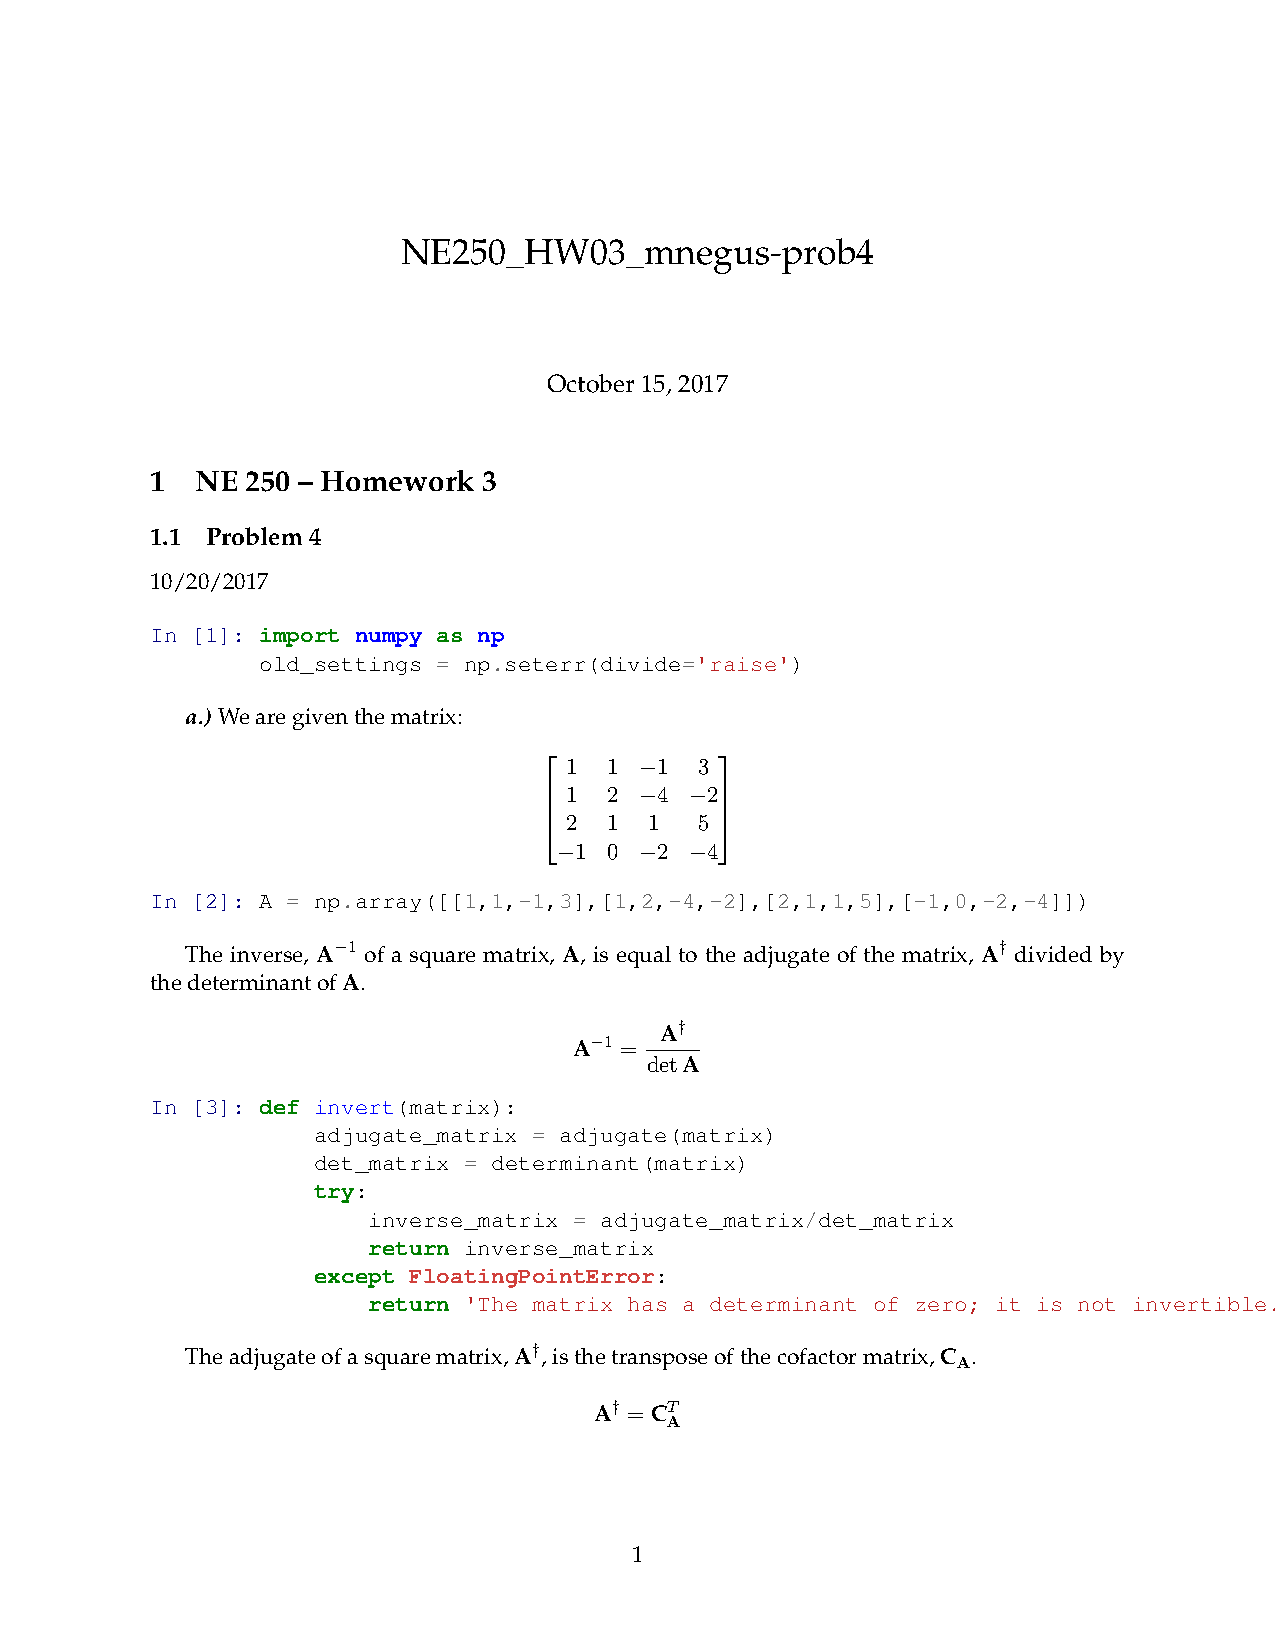
\includepdf[pages=-]{NE250_HW03_mnegus-prob4.pdf}
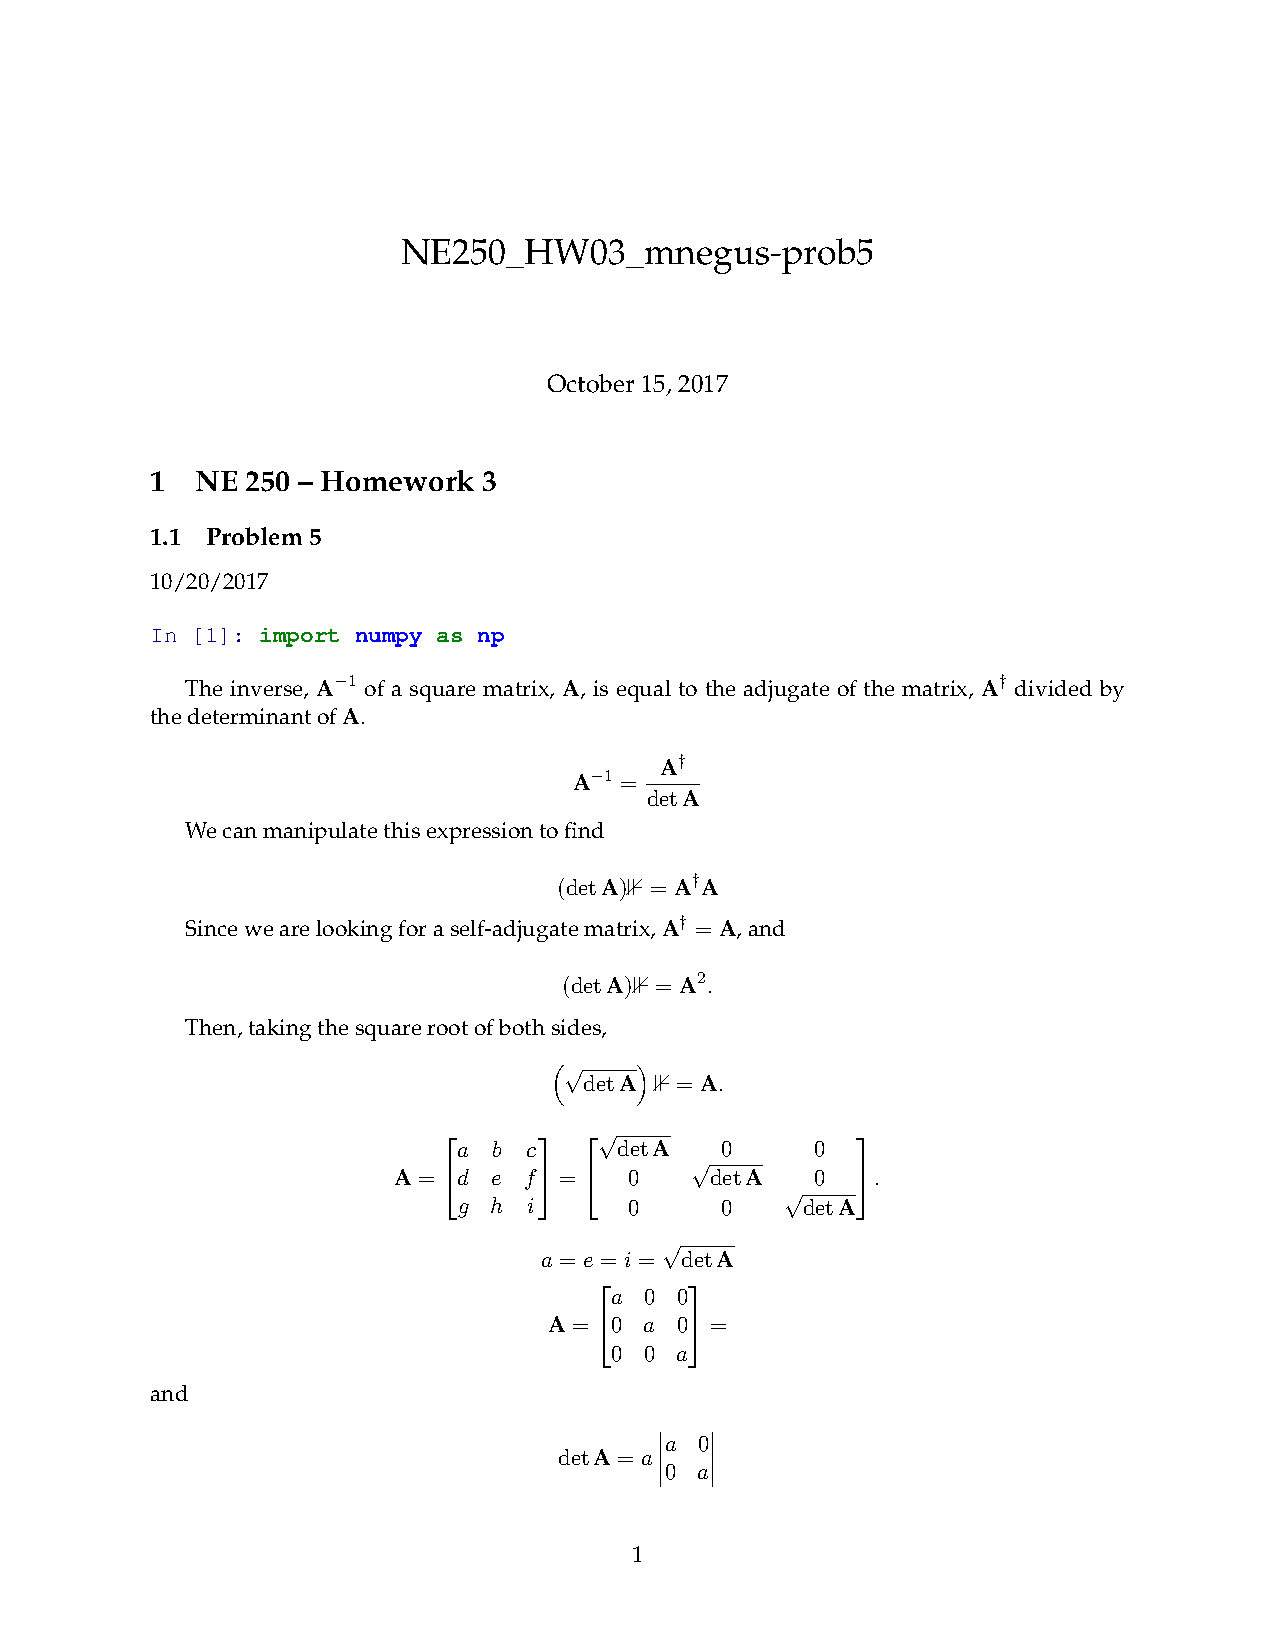
\includepdf[pages=-]{NE250_HW03_mnegus-prob5.pdf}


\end{document}








 
